\documentclass[aspectratio=1610]{beamer}
\usepackage[T1]{fontenc}
\usetheme{wildcat}
\usetikzlibrary{arrows.meta,angles,quotes,calc,intersections,positioning}

\usepackage{amsmath,amssymb,amsfonts}
\usepackage{booktabs}
\usepackage{relsize}
\usepackage{pgfplots}
\pgfplotsset{compat=1.16}
\usepackage{array}
\usepackage{siunitx}
\usepackage{cancel}
\usepackage{jupyter}
\usepackage{minted}

\let\oldfootnotesize\footnotesize
\renewcommand*{\footnotesize}{\oldfootnotesize\tiny}

\def\mathdefault#1{#1}
\everymath=\expandafter{\the\everymath\displaystyle}


\title{Reactivity: Units, \\ Coefficients, and Control \\
       {\small\it NE 630 - Lecture 20}}

\date{\input{term.txt} \\ {\footnotesize Git SHA: \input{git_sha.txt}}}

\author{Jeremy Roberts}


\definecolor{ksupurple}{HTML}{512888}
\definecolor{orange}{HTML}{CA7C1B}
\definecolor{skyblue}{RGB}{180,220,255}

\begin{document}

\begin{frame}
\titlepage
\end{frame}
 
 
%%%%%%%%%%%%%%%%%%%%%%%%%%%%%%%%%%%%%%%%%%%%%%%%%%%
\begin{frame}{Primary Objective}

Students will be able to 

\vfill

\begin{quote}
\textcolor{wcprimary}{quantify changes in reactivity due to changes in operating conditions.
}
\end{quote}

\vfill 

\end{frame}

%%%%%%%%%%%%%%%%%%%%%%%%%%%%%%%%%%%%%%%%%%%%%%%%%%%%%%%%%%%%%%%%%%%%%%%%%%%%%%
\begin{frame}[fragile]{Review: OpenMC and the PWR Unit Cell}
 
If you are on Beocat, there should be no problems with the example as given.
However, if you are on Docker, the included data is actually a bit 
incomplete.  

\vfill 

First, add the following {\bf at the top of your notebook} to avoid any errors related to missing nuclides:
\begin{minted}[frame=single,framesep=5pt]{python}
import os
os.environ["OPENMC_CROSS_SECTIONS"] = \
  "/root/nndc_hdf5/cross_sections.xml"
\end{minted}

\vfill 

Then, because the data included is only available for 294 K, you cannot set other temperatures!  Sorry :(

\end{frame}


%%%%%%%%%%%%%%%%%%%%%%%%%%%%%%%%%%%%%%%%%%%%%%%%%%%%%%%%%%%%%%%%%%%%%%%%%%%%%%
\begin{frame}[fragile]{Reactivity}
 
Recall that

\begin{equation*}
  k_{\infty} = \frac{\text{total production rate}}{\text{total absorption rate}} \, .
\end{equation*}

\vfill 

Then the {\bf reactivity} is defined as

\begin{equation*}
  \rho_{\infty} = \frac{k_{\infty} - 1}{k_{\infty}} \, 
  \tag{Like FNRP  9.1}
\end{equation*}

\vfill 

{\bf Example}.  Compute the reactivity of a reactor with $k_{\infty} = 1.01$.

\pause 

{\small {\bf Ans}. $\rho_{\infty} = 0.00990$.}
 
\end{frame}

 


%%%%%%%%%%%%%%%%%%%%%%%%%%%%%%%%%%%%%%%%%%%%%%%%%%%%%%%%%%%%%%%%%%%%%%%%%%%%%%
\begin{frame}[fragile]{Reactivity Units}

Although $\rho$ (and $k$) are unitless, the small magnitude of 
reactivities suggests different units.  By example, these are 
\begin{align*}
 \rho    &= 0.00990 \, (\Delta k/k) \\
               &= 0.990 \, (\% \Delta k/k) \\ 
               &= 990 \, (\text{pcm}) \, ,
\end{align*}
where ``pcm'' stands for ``percent milli'' (or, $1$ part in $10^5$).

\vfill  
\pause 

An alternative unit used by operators is the {\it dollar} of reactivity.
Given the {\bf delayed neutron precursor fraction} $\beta$, we say that\footnote{Because $\beta$ depends on the fissioning species, reactivities reported in dollars are generally specific to the particular system!} 
\begin{equation*}
    \rho \, (\Delta k/k) = \frac{\rho}{\beta} \, (\$) \, .
\end{equation*}

{\bf Example}:  If $\beta = 0.007$, what is $\rho$ in \$?

\pause 

{\small {\bf Ans.}  $0.0099/0.007 = 1.4\$ $.}

\end{frame}


%%%%%%%%%%%%%%%%%%%%%%%%%%%%%%%%%%%%%%%%%%%%%%%%%%%%%%%%%%%%%%%%%%%%%%%%%%%%%%
\begin{frame}[fragile]{Reactivity Units}

Although $\rho$ (and $k$) are unitless, the small magnitude of 
reactivities suggests different units.  By example, these are 
\begin{align*}
 \rho    &= 0.00990 \, (\Delta k/k) \\
               &= 0.990 \, (\% \Delta k/k) \\ 
               &= 990 \, (\text{pcm}) \, ,
\end{align*}
where ``pcm'' stands for ``percent milli'' (or, $1$ part in $10^5$).

\vfill  
\pause 

An alternative unit used by operators is the {\it dollar} of reactivity.
Given the {\bf delayed neutron precursor fraction} $\beta$, we say that\footnote{Because $\beta$ depends on the fissioning species, reactivities reported in dollars are generally specific to the particular system!} 
\begin{equation*}
    \rho \, (\Delta k/k) = \frac{\rho}{\beta} \, (\$) \, .
\end{equation*}

{\bf Example}:  If $\beta = 0.007$, what is $\rho$ in \$?

\pause 

{\small {\bf Ans.}  $0.0099/0.007 = 1.4\$ $.}

\end{frame}


%%%%%%%%%%%%%%%%%%%%%%%%%%%%%%%%%%%%%%%%%%%%%%%%%%%%%%%%%%%%%%%%%%%%%%%%%%%%%%
\begin{frame}[fragile]{Excess Reactivity and Control}

Reactors must have a positive or {\bf excess reactivity} to operate; otherwise, the first fission would bring an initial $\rho = 0$ to $\rho < 0$!  To  maintain a critical state, some form of adjustable {\bf reactivity control} is used to decrease (or increase) $\rho$ to balance  \textcolor{wcprimary}{short-} and \textcolor{wcalerted}{long-term} changes in the operating conditions that include 
\begin{itemize}
 \item \textcolor{wcprimary}{temperature (of the fuel)}
 \item \textcolor{wcprimary}{density (of the coolant)}
 \item \textcolor{wcprimary}{control configuration (e.g., soluble boron concentration; rod positions)}
 \item \textcolor{wcalerted}{xenon (from zero to equilibrium)}
 \item \textcolor{wcalerted}{depletion (we lose ${}^{235}$U with each fission)}
\end{itemize}

\vfill

The impact of these changes on $\rho$ are characterized via
\begin{itemize}
 \item reactivity worths $\Delta \rho$ (e.g., power defect)
 \item reactivity coefficients $\alpha_x = \frac{\partial \rho}{\partial x}\Big |_{\text{non-}x\text{ fixed}}$ (e.g., $x = T_F$)
\end{itemize}

\end{frame}

%%%%%%%%%%%%%%%%%%%%%%%%%%%%%%%%%%%%%%%%%%%%%%%%%%%%%%%%%%%%%%%%%%%%%%%%%%%%%%
\begin{frame}[fragile]{Excess Reactivity from Shutdown to Full Power}
 
\begin{columns}[T,onlytextwidth]

\begin{column}{0.5\textwidth}

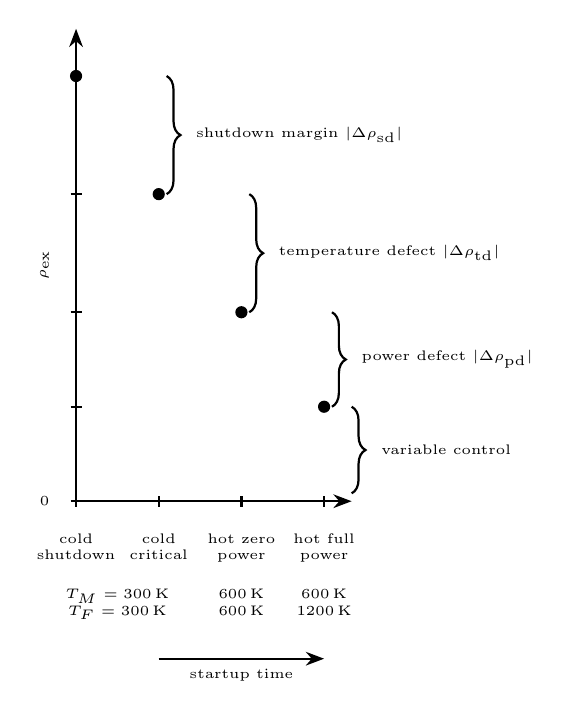
\begin{tikzpicture}[
  >=Stealth,
  thick,
  dot/.style={circle,fill,inner sep=2pt},
  lab/.style={font=\footnotesize},
  every node/.style={ }
]

% --- x locations for the four conditions
\def\xMin{0} 
\def\xMax{3.5} 
\def\xA{0.0*\xMax}   % cold shutdown
\def\xB{0.3*\xMax}   % cold critical
\def\xC{0.6*\xMax}   % hot zero power
\def\xD{0.9*\xMax}   % full power


% --- y values of the excess-reactivity curve (adjust to taste)
\def\yMax{6.0}
\def\yMin{0.0}
\def\yA{0.9*\yMax}
\def\yB{0.65*\yMax}
\def\yC{0.4*\yMax}
\def\yD{0.2*\yMax}

% --- Axes
\draw[->] (\xMin,\yMin) -- (\xMax,\yMin);
\draw[->] (\xMin,\yMin) -- (\xMin,\yMax);
\node[lab, rotate=90] at (-0.4, 3) {$\rho_{\text{ex}}$};
\node[lab] at (-0.4, \yMin) {$0$};

% --- Zero markers under each operating condition
%\foreach \x in {\xA,\xB,\xC,\xD}{\fill (\x,0) circle (2.2pt);}

\foreach \x in  {\xA,\xB,\xC,\xD}
   \draw [shift={(\x,0)}, color=black] (0pt,-2pt) -- (0pt,2pt);
   
\foreach \y in  {\yMin, \yA,\yB,\yC,\yD}
   \draw [shift={(0,\y)}, color=black] (-2pt,0pt) -- (2pt,0pt);

% --- Trend line (dashed) and the four points
%\draw[dashed] (\xA,\yA) -- (\xD,\yD);
\fill (\xA,\yA) circle (2.2pt);
\fill (\xB,\yB) circle (2.2pt);
\fill (\xC,\yC) circle (2.2pt);
\fill (\xD,\yD) circle (2.2pt);

% --- Braces and labels
% Shutdown margin: between cold-shutdown dot and cold-critical point
\draw[decorate,decoration={brace,amplitude=5pt,mirror}]
      (\xB+0.1,\yB) -- node[right=7pt,lab]{shutdown margin $|\Delta \rho_{\text{sd}}|$} (\xB+0.1,\yA);

% Temperature defect: cold critical -> hot zero power
\draw[decorate,decoration={brace,amplitude=5pt,mirror}]
      (\xC+0.1,\yC) -- node[right=7pt,lab]{temperature defect $|\Delta \rho_{\text{td}}|$} (\xC+0.1,\yB);

% Power defect: hot zero power -> full power
\draw[decorate,decoration={brace,amplitude=5pt,mirror}]
      (\xD+0.1,\yD) -- node[right=7pt,lab]{power defect $|\Delta \rho_{\text{pd}}|$} (\xD+0.1,\yC);

% "How to handle?" from zero to the full-power point
\draw[decorate,decoration={brace,amplitude=5pt,mirror}]
      (\xMax,\yMin+0.1) -- node[right=7pt,lab]{variable control} (\xMax,\yD);

% --- Operating-condition labels
\node[below=8pt,align=center,lab] at (\xA,0) {cold\\shutdown};
\node[below=8pt,align=center,lab] at (\xB,0) {cold\\critical};
\node[below=8pt,align=center,lab] at (\xC,0) {hot zero\\power};
\node[below=8pt,align=center,lab] at (\xD,0) {hot full\\power};

% --- Temperature annotations
\node[below=28pt,lab,align=center] at ({(\xA+\xB)/2},0)
  {$T_M=300\,\text{K}$\\$T_F=300\,\text{K}$};
\node[below=28pt,lab,align=center] at (\xC,0)
  {$600\, \text{K}$\\$600\,\text{K}$};
\node[below=28pt,lab,align=center] at (\xD,0)
  {$600\,\mathrm{K}$\\$1200\,\mathrm{K}$};

% --- Startup time arrow
\draw[->] (\xB,-2) -- node[below,lab]{startup time} (\xD,-2);

\end{tikzpicture}

\end{column}

\begin{column}{0.5\textwidth}

 

$\Delta\rho_{\text{sd}}$: Amount by which reactor is subcritical with all control rods inserted.  The total control-rod worth is $\Delta \rho_{\text{ex}}+|\Delta \rho_{\text{sd}}|$.

\vspace{0.25cm}

$\Delta\rho_{\text{td}}$: Negative change in reactivity when core goes from 300 K to 600 K due to fuel Doppler broadening and moderator density reduction.


\vspace{0.25cm}


$\Delta\rho_{\text{pd}}$: Additional negative reactivity inserted as power increases from hot zero power to full power, further shifting temperature and density.

\vspace{0.25cm}


Variable control: soluble boron or control rods bring $\rho_{\text{ex}}$ to 0. 

\vspace{0.25cm}



\end{column}

\end{columns}

\end{frame}

%%%%%%%%%%%%%%%%%%%%%%%%%%%%%%%%%%%%%%%%%%%%%%%%%%%%%%%%%%%%%%%%%%%%%%%%%%%%%%
\begin{frame}[fragile]{Understanding $\alpha_x$ Through the Four Factors}

The instantaneous change in $\rho$ due to a change in some 
system parameter $x$ (with all other parameters fixed) is

\begin{align*}
 \alpha_x = \frac{\partial \rho}{\partial x}
 \approx \frac{1}{k} \frac{\partial k}{\partial x}  
 = \frac{1}{\eta_T} \frac{\partial \eta_T}{\partial x}
  + \frac{1}{f} \frac{\partial f}{\partial x}
  + \frac{1}{p} \frac{\partial p}{\partial x}
  + \frac{1}{\varepsilon} \frac{\partial \varepsilon}{\partial x}
\end{align*}

where $x \in \{T_F, T_M, \ldots \}$.  

\vfill 

The most important coefficients of reactivity are

\begin{equation*}
 \alpha_F = \text{fuel temperature coefficient (FTC)}
\end{equation*}
and
\begin{equation*}
 \alpha_M = \text{moderator temperature coefficient (MTC)} \, .
\end{equation*}

\vfill 

{\bf Ponderable}.  Which of the four factors explicitly depend 
on $T_F$?  $T_M$?

\end{frame}

%%%%%%%%%%%%%%%%%%%%%%%%%%%%%%%%%%%%%%%%%%%%%%%%%%%%%%%%%%%%%%%%%%%%%%%%%%%%%%
\begin{frame}[fragile]{Fuel Temperature Coefficient}

Recall for a UO$_2$ fuel element of mass density $\rho$ and diameter $D$ that 
\begin{equation*}
\tag{FNRP 4.40}
p(T_F) = e^{-\displaystyle\frac{V_f N_{fe} I_{\text{het}}(T_F)}{V_m \xi^m \bar{\Sigma}_s^m}} \, ,
\end{equation*}
where we write $p$ as a function of $T_F$, and 
\begin{align*}
\tag{FNRP 9.13}
 I_{\text{het}}(T_F) = I_{\text{het}}(300) [ 1 + \tilde{\gamma} (\sqrt{T_F} - \sqrt{300})] \\
\tag{FNRP Table 4.3}
 I_{\text{het}}(300) = 4.45 + 26.6\sqrt{4/(\rho D)} \\
\tag{FNRP 9.14 and Table 9.1}
 \tilde{\gamma} = 0.0061 + 0.0047(4/(\rho D)) \, .
\end{align*}

\pause 
\vfill 

Since $p$ is the only factor with (explicit) $T_F$ dependence, we have 
\begin{align*}
\tag{FNRP 9.16}
  \alpha_F = \frac{1}{p} \frac{\partial p}{\partial T_F} 
    = -\ln{\left ( \frac{1}{p(300)} \right ) }\frac{\tilde{\gamma}}{2\sqrt{T_F}} \, .
\end{align*}

\vfill 

For PWR's, $|\alpha_F| \approx 2--3$ pcm/K, while for our TRIGA, $|\alpha_F| \approx -10$ pcm/K!

\end{frame}


%%%%%%%%%%%%%%%%%%%%%%%%%%%%%%%%%%%%%%%%%%%%%%%%%%%%%%%%%%%%%%%%%%%%%%%%%%%%%%
\begin{frame}[fragile]{Moderator Temperature Coefficient}

Further, recall that 
\begin{equation*}
 f = \frac{1}{1 + \varsigma\left ( \frac{V_m}{V_f} \frac{\bar{\Sigma}^m_{aT}}{\bar{\Sigma}^f_{aT}} \right )}
\end{equation*}
Both $p$ and $f$ depend on $T_m$ through the moderator densitites: 
if $\rho_{\text{H}_2\text{O}} \downarrow$, then $\bar{\Sigma}^m_{aT}\downarrow$ and $\xi^m \bar{\Sigma}_s^m \downarrow$.

\vfill 
Based on our simple models for $p$ and $f$, the net result is 
\begin{equation*}
\tag{FNRP 9.XX}
 \alpha_{M}
  = -\beta_M \left ( \textcolor{wcprimary}{\ln(1/p)} - \textcolor{wcalerted}{(1-f)} \right) \, ,
\end{equation*}
where $\beta_M$ is the volumetric coefficient of thermal expansion of the moderator.  To ensure $\alpha_M < 0$ (negative feedback) requires that
$\textcolor{wcprimary}{\ln(1/p)} > \textcolor{wcalerted}{(1-f)}$.

\vfill 

{\bf Example}. If $p=0.6$, $f=0.95$, and $\beta_M \approx 2.9\cdot 10^{-4} \si{\per\kelvin}$, determine $\alpha_M$.
\pause 

{\small {\bf Ans}. $\alpha_M = -2.9\cdot 10^{-4} (\ln(1/0.6) - (1-0.95) \approx -13$ pcm/K}.

\end{frame}

%%%%%%%%%%%%%%%%%%%%%%%%%%%%%%%%%%%%%%%%%%%%%%%%%%%%%%%%%%%%%%%%%%%%%%%%%%%%%
\begin{frame}[fragile]{Addendum: On the Use of OpenMC for $\alpha_x$}

Perhaps the easiest way to approximate, e.g., $\alpha_F$ is by using a 
{\bf finite-difference approximation}.  Suppose we run our PWR unit cell 
model with a fuel temperature at 1200 K and get $k_{1200}$.  Doing the 
same for $T_F = 1300$ K, we get $k_{1300}$.  It follows that
\begin{equation*}
 \alpha_F \approx \frac{\rho_{1300}-\rho_{1200}}{1300-1200} \, .
\end{equation*}
Note, however, that the uncertainties in $k$ can easily be on the order of
several pcm, so it's very easy for $\alpha_F$ to have overwhelmingly large
relative errors!

\vfill

Finally, most Monte Carlo tools, including OpenMC, provide microscopic cross sections 
that are evaluated at several fixed temperatures that span conditions of 
interest.  How values are produced at intermediate temperatures depends on 
the tool; by default, OpenMC uses interpolation, which might not be accurate enough 
to capture the impact of Doppler broadening!

\end{frame}

\end{document}

